
%% bare_conf.tex
%% V1.4b
%% 2015/08/26
%% by Michael Shell
%% See:
%% http://www.michaelshell.org/
%% for current contact information.
%%
%% This is a skeleton file demonstrating the use of IEEEtran.cls
%% (requires IEEEtran.cls version 1.8b or later) with an IEEE
%% conference paper.
%%
%% Support sites:
%% http://www.michaelshell.org/tex/ieeetran/
%% http://www.ctan.org/pkg/ieeetran
%% and
%% http://www.ieee.org/

%%*************************************************************************
%% Legal Notice:
%% This code is offered as-is without any warranty either expressed or
%% implied; without even the implied warranty of MERCHANTABILITY or
%% FITNESS FOR A PARTICULAR PURPOSE! 
%% User assumes all risk.
%% In no event shall the IEEE or any contributor to this code be liable for
%% any damages or losses, including, but not limited to, incidental,
%% consequential, or any other damages, resulting from the use or misuse
%% of any information contained here.
%%
%% All comments are the opinions of their respective authors and are not
%% necessarily endorsed by the IEEE.
%%
%% This work is distributed under the LaTeX Project Public License (LPPL)
%% ( http://www.latex-project.org/ ) version 1.3, and may be freely used,
%% distributed and modified. A copy of the LPPL, version 1.3, is included
%% in the base LaTeX documentation of all distributions of LaTeX released
%% 2003/12/01 or later.
%% Retain all contribution notices and credits.
%% ** Modified files should be clearly indicated as such, including  **
%% ** renaming them and changing author support contact information. **
%%*************************************************************************


% *** Authors should verify (and, if needed, correct) their LaTeX system  ***
% *** with the testflow diagnostic prior to trusting their LaTeX platform ***
% *** with production work. The IEEE's font choices and paper sizes can   ***
% *** trigger bugs that do not appear when using other class files.       ***                          ***
% The testflow support page is at:
% http://www.michaelshell.org/tex/testflow/



\documentclass[conference]{IEEEtran}
% Some Computer Society conferences also require the compsoc mode option,
% but others use the standard conference format.
%
% If IEEEtran.cls has not been installed into the LaTeX system files,
% manually specify the path to it like:
% \documentclass[conference]{../sty/IEEEtran}





% Some very useful LaTeX packages include:
% (uncomment the ones you want to load)


% *** MISC UTILITY PACKAGES ***
%
%\usepackage{ifpdf}
% Heiko Oberdiek's ifpdf.sty is very useful if you need conditional
% compilation based on whether the output is pdf or dvi.
% usage:
% \ifpdf
%   % pdf code
% \else
%   % dvi code
% \fi
% The latest version of ifpdf.sty can be obtained from:
% http://www.ctan.org/pkg/ifpdf
% Also, note that IEEEtran.cls V1.7 and later provides a builtin
% \ifCLASSINFOpdf conditional that works the same way.
% When switching from latex to pdflatex and vice-versa, the compiler may
% have to be run twice to clear warning/error messages.






% *** CITATION PACKAGES ***
%
%\usepackage{cite}
% cite.sty was written by Donald Arseneau
% V1.6 and later of IEEEtran pre-defines the format of the cite.sty package
% \cite{} output to follow that of the IEEE. Loading the cite package will
% result in citation numbers being automatically sorted and properly
% "compressed/ranged". e.g., [1], [9], [2], [7], [5], [6] without using
% cite.sty will become [1], [2], [5]--[7], [9] using cite.sty. cite.sty's
% \cite will automatically add leading space, if needed. Use cite.sty's
% noadjust option (cite.sty V3.8 and later) if you want to turn this off
% such as if a citation ever needs to be enclosed in parenthesis.
% cite.sty is already installed on most LaTeX systems. Be sure and use
% version 5.0 (2009-03-20) and later if using hyperref.sty.
% The latest version can be obtained at:
% http://www.ctan.org/pkg/cite
% The documentation is contained in the cite.sty file itself.






% *** GRAPHICS RELATED PACKAGES ***
%
\ifCLASSINFOpdf
  \usepackage[pdftex]{graphicx}
  % declare the path(s) where your graphic files are
  % \graphicspath{{../pdf/}{../jpeg/}}
  % and their extensions so you won't have to specify these with
  % every instance of \includegraphics
  \DeclareGraphicsExtensions{.pdf,.jpeg,.png}
\else
  % or other class option (dvipsone, dvipdf, if not using dvips). graphicx
  % will default to the driver specified in the system graphics.cfg if no
  % driver is specified.
  % \usepackage[dvips]{graphicx}
  % declare the path(s) where your graphic files are
  % \graphicspath{{../eps/}}
  % and their extensions so you won't have to specify these with
  % every instance of \includegraphics
  % \DeclareGraphicsExtensions{.eps}
\fi
% graphicx was written by David Carlisle and Sebastian Rahtz. It is
% required if you want graphics, photos, etc. graphicx.sty is already
% installed on most LaTeX systems. The latest version and documentation
% can be obtained at: 
% http://www.ctan.org/pkg/graphicx
% Another good source of documentation is "Using Imported Graphics in
% LaTeX2e" by Keith Reckdahl which can be found at:
% http://www.ctan.org/pkg/epslatex
%
% latex, and pdflatex in dvi mode, support graphics in encapsulated
% postscript (.eps) format. pdflatex in pdf mode supports graphics
% in .pdf, .jpeg, .png and .mps (metapost) formats. Users should ensure
% that all non-photo figures use a vector format (.eps, .pdf, .mps) and
% not a bitmapped formats (.jpeg, .png). The IEEE frowns on bitmapped formats
% which can result in "jaggedy"/blurry rendering of lines and letters as
% well as large increases in file sizes.
%
% You can find documentation about the pdfTeX application at:
% http://www.tug.org/applications/pdftex





% *** MATH PACKAGES ***
%
%\usepackage{amsmath}
% A popular package from the American Mathematical Society that provides
% many useful and powerful commands for dealing with mathematics.
%
% Note that the amsmath package sets \interdisplaylinepenalty to 10000
% thus preventing page breaks from occurring within multiline equations. Use:
%\interdisplaylinepenalty=2500
% after loading amsmath to restore such page breaks as IEEEtran.cls normally
% does. amsmath.sty is already installed on most LaTeX systems. The latest
% version and documentation can be obtained at:
% http://www.ctan.org/pkg/amsmath





% *** SPECIALIZED LIST PACKAGES ***
%
%\usepackage{algorithmic}
% algorithmic.sty was written by Peter Williams and Rogerio Brito.
% This package provides an algorithmic environment fo describing algorithms.
% You can use the algorithmic environment in-text or within a figure
% environment to provide for a floating algorithm. Do NOT use the algorithm
% floating environment provided by algorithm.sty (by the same authors) or
% algorithm2e.sty (by Christophe Fiorio) as the IEEE does not use dedicated
% algorithm float types and packages that provide these will not provide
% correct IEEE style captions. The latest version and documentation of
% algorithmic.sty can be obtained at:
% http://www.ctan.org/pkg/algorithms
% Also of interest may be the (relatively newer and more customizable)
% algorithmicx.sty package by Szasz Janos:
% http://www.ctan.org/pkg/algorithmicx




% *** ALIGNMENT PACKAGES ***
%
%\usepackage{array}
% Frank Mittelbach's and David Carlisle's array.sty patches and improves
% the standard LaTeX2e array and tabular environments to provide better
% appearance and additional user controls. As the default LaTeX2e table
% generation code is lacking to the point of almost being broken with
% respect to the quality of the end results, all users are strongly
% advised to use an enhanced (at the very least that provided by array.sty)
% set of table tools. array.sty is already installed on most systems. The
% latest version and documentation can be obtained at:
% http://www.ctan.org/pkg/array


% IEEEtran contains the IEEEeqnarray family of commands that can be used to
% generate multiline equations as well as matrices, tables, etc., of high
% quality.




% *** SUBFIGURE PACKAGES ***
\ifCLASSOPTIONcompsoc
  \usepackage[caption=false,font=normalsize,labelfont=sf,textfont=sf]{subfig}
\else
  \usepackage[caption=false,font=footnotesize]{subfig}
\fi
% subfig.sty, written by Steven Douglas Cochran, is the modern replacement
% for subfigure.sty, the latter of which is no longer maintained and is
% incompatible with some LaTeX packages including fixltx2e. However,
% subfig.sty requires and automatically loads Axel Sommerfeldt's caption.sty
% which will override IEEEtran.cls' handling of captions and this will result
% in non-IEEE style figure/table captions. To prevent this problem, be sure
% and invoke subfig.sty's "caption=false" package option (available since
% subfig.sty version 1.3, 2005/06/28) as this is will preserve IEEEtran.cls
% handling of captions.
% Note that the Computer Society format requires a larger sans serif font
% than the serif footnote size font used in traditional IEEE formatting
% and thus the need to invoke different subfig.sty package options depending
% on whether compsoc mode has been enabled.
%
% The latest version and documentation of subfig.sty can be obtained at:
% http://www.ctan.org/pkg/subfig




% *** FLOAT PACKAGES ***
%
%\usepackage{fixltx2e}
% fixltx2e, the successor to the earlier fix2col.sty, was written by
% Frank Mittelbach and David Carlisle. This package corrects a few problems
% in the LaTeX2e kernel, the most notable of which is that in current
% LaTeX2e releases, the ordering of single and double column floats is not
% guaranteed to be preserved. Thus, an unpatched LaTeX2e can allow a
% single column figure to be placed prior to an earlier double column
% figure.
% Be aware that LaTeX2e kernels dated 2015 and later have fixltx2e.sty's
% corrections already built into the system in which case a warning will
% be issued if an attempt is made to load fixltx2e.sty as it is no longer
% needed.
% The latest version and documentation can be found at:
% http://www.ctan.org/pkg/fixltx2e


%\usepackage{stfloats}
% stfloats.sty was written by Sigitas Tolusis. This package gives LaTeX2e
% the ability to do double column floats at the bottom of the page as well
% as the top. (e.g., "\begin{figure*}[!b]" is not normally possible in
% LaTeX2e). It also provides a command:
%\fnbelowfloat
% to enable the placement of footnotes below bottom floats (the standard
% LaTeX2e kernel puts them above bottom floats). This is an invasive package
% which rewrites many portions of the LaTeX2e float routines. It may not work
% with other packages that modify the LaTeX2e float routines. The latest
% version and documentation can be obtained at:
% http://www.ctan.org/pkg/stfloats
% Do not use the stfloats baselinefloat ability as the IEEE does not allow
% \baselineskip to stretch. Authors submitting work to the IEEE should note
% that the IEEE rarely uses double column equations and that authors should try
% to avoid such use. Do not be tempted to use the cuted.sty or midfloat.sty
% packages (also by Sigitas Tolusis) as the IEEE does not format its papers in
% such ways.
% Do not attempt to use stfloats with fixltx2e as they are incompatible.
% Instead, use Morten Hogholm'a dblfloatfix which combines the features
% of both fixltx2e and stfloats:
%
% \usepackage{dblfloatfix}
% The latest version can be found at:
% http://www.ctan.org/pkg/dblfloatfix




% *** PDF, URL AND HYPERLINK PACKAGES ***
%
%\usepackage{url}
% url.sty was written by Donald Arseneau. It provides better support for
% handling and breaking URLs. url.sty is already installed on most LaTeX
% systems. The latest version and documentation can be obtained at:
% http://www.ctan.org/pkg/url
% Basically, \url{my_url_here}.




% *** Do not adjust lengths that control margins, column widths, etc. ***
% *** Do not use packages that alter fonts (such as pslatex).         ***
% There should be no need to do such things with IEEEtran.cls V1.6 and later.
% (Unless specifically asked to do so by the journal or conference you plan
% to submit to, of course. )


% correct bad hyphenation here
\hyphenation{op-tical net-works semi-conduc-tor}


\begin{document}
%
% paper title
% Titles are generally capitalized except for words such as a, an, and, as,
% at, but, by, for, in, nor, of, on, or, the, to and up, which are usually
% not capitalized unless they are the first or last word of the title.
% Linebreaks \\ can be used within to get better formatting as desired.
% Do not put math or special symbols in the title.
\title{An Evolutionary Algorithm For Online\\ Spatial Discretization Optimization}


% author names and affiliations
% use a multiple column layout for up to three different
% affiliations
\author{\IEEEauthorblockN{Edward Norris}
\IEEEauthorblockA{Missouri University of Science and Technology\\
Rolla, Missouri\\
Email: etnc6d@mst.edu}}
%\and
%\IEEEauthorblockN{Homer Simpson}
%\IEEEauthorblockA{Twentieth Century Fox\\
%Springfield, USA\\
%Email: homer@thesimpsons.com}
%\and
%\IEEEauthorblockN{James Kirk\\ and Montgomery Scott}
%\IEEEauthorblockA{Starfleet Academy\\
%San Francisco, California 96678--2391\\
%Telephone: (800) 555--1212\\
%Fax: (888) 555--1212}}

% conference papers do not typically use \thanks and this command
% is locked out in conference mode. If really needed, such as for
% the acknowledgment of grants, issue a \IEEEoverridecommandlockouts
% after \documentclass

% for over three affiliations, or if they all won't fit within the width
% of the page, use this alternative format:
% 
%\author{\IEEEauthorblockN{Michael Shell\IEEEauthorrefmark{1},
%Homer Simpson\IEEEauthorrefmark{2},
%James Kirk\IEEEauthorrefmark{3}, 
%Montgomery Scott\IEEEauthorrefmark{3} and
%Eldon Tyrell\IEEEauthorrefmark{4}}
%\IEEEauthorblockA{\IEEEauthorrefmark{1}School of Electrical and Computer Engineering\\
%Georgia Institute of Technology,
%Atlanta, Georgia 30332--0250\\ Email: see http://www.michaelshell.org/contact.html}
%\IEEEauthorblockA{\IEEEauthorrefmark{2}Twentieth Century Fox, Springfield, USA\\
%Email: homer@thesimpsons.com}
%\IEEEauthorblockA{\IEEEauthorrefmark{3}Starfleet Academy, San Francisco, California 96678-2391\\
%Telephone: (800) 555--1212, Fax: (888) 555--1212}
%\IEEEauthorblockA{\IEEEauthorrefmark{4}Tyrell Inc., 123 Replicant Street, Los Angeles, California 90210--4321}}




% use for special paper notices
%\IEEEspecialpapernotice{(Invited Paper)}




% make the title area
\maketitle

% As a general rule, do not put math, special symbols or citations
% in the abstract
\begin{abstract}
The abstract goes here.
\end{abstract}

% no keywords
\begin{IEEEkeywords}
help
\end{IEEEkeywords}

% For peer review papers, you can put extra information on the cover
% page as needed:
% \ifCLASSOPTIONpeerreview
% \begin{center} \bfseries EDICS Category: 3-BBND \end{center}
% \fi
%
% For peerreview papers, this IEEEtran command inserts a page break and
% creates the second title. It will be ignored for other modes.
\IEEEpeerreviewmaketitle



\section{Introduction}
Monte Carlo simulations require detailed knowledge of the geometry of a system as well as type and location of radiation. With this information, a Monte Carlo simulation can calculate the dose to a person at a particular location due to the radioactive source(s). Radiation penetration through a shield is described as a Poisson process, meaning that the accuracy of a Monte Carlo simulation within some volume is inversely proportional to the square root of the number of particles in that volume. Therefore, with deep shielding problems, in which a strong source is attenuated greatly (reduced in strength), the statistical uncertainty increases dramatically. 

In order to alleviate the high uncertainty in the analog Monte Carlo (so called due to it being directly analogous to the physical transport process), biasing parameters are added to Monte Carlo simulations. Biasing parameters split important particles and kill unimportant ones to maximize the number of particles that reach the area of interest and reduce the computational overhead of tracking those that do not.

However, the production of accurate biasing parameters remains difficult. To remedy this, an adjoint transport calculation is made using a deterministic code. Rather than tracking particles forward through time as they traverse space and building a mesh of dose values, the adjoint solution tracks particles backward from an object of interest and builds a mesh of \textit{importance} to the region of interest.

Quantification of the effectiveness of a set of biasing parameters is done by calculating the figure of merit (FOM). The FOM is a metric used to compare the overall performance of two simulations and gives a directly comparable measure of performance for any two simulations provided that the physical problem being solved does not change and the computation hardware the two simulations were run on are identical. The FOM is defined in Eq.~\ref{eq:fom} where $T$ is the wall clock runtime of the simulation and $R$ is the estimated relative uncertainty of the output.
\begin{equation} \label{eq:fom}
FOM = \frac{1}{T R^2}
\end{equation}
Systems that use a deterministic solver to calculate the adjoint solution in order to produce biasing parameters for the primary Monte Carlo simulation are known as hybrid systems. One such system is AutomateD VAriaNce reducTion Generator (ADVANTG)~\cite{ref:Mosher2015} which is a framework developed at Oak Ridge National Laboratory specifically to produce biasing parameters for Monte Carlo N-Particle version~5 (MCNP)~\cite{ref:X5}, a Monte Carlo code developed by Los Alamos National Laboratory for radiation transport. 

However, currently available general-purpose radiation transport hybrid systems require a user defined spatial discretization in the form of a Cartesian grid~\cite{ref:Wagner2014, ref:Mosher2015}. This work will develop an evolutionary algorithm (EA) to optimize the spatial discretization grid for ADVANTG which will accelerate MCNP; these two codes have been coupled together very successfully~\cite{ref:Blakeman2007, ref:Risner2013, ref:Ibrahim2011, ref:Wagner2011}.

\section{Background}
In modern deterministic algorithms, spatial refinement is performed with a quadtree in 2D or an octree in 3D. However, quadtree/octree geometries cannot be utilized in the ADVANTG framework, instead, a structured Cartesian grid is required. A comparison of a 2D quadtree geometry and a 2D structured grid is shown in Fig.~\ref{fig:treecomp}. 

\begin{figure*}[!t]
\centering
\subfloat[Case I]{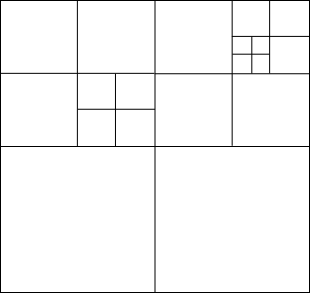
\includegraphics[width=2.5in]{treecomp_quad}
\label{fig:treecompa}}
\hfil
\subfloat[Case II]{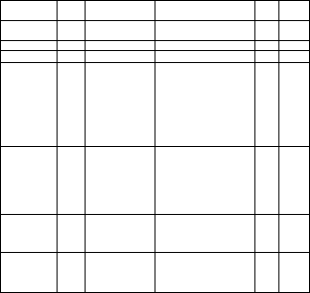
\includegraphics[width=2.5in]{treecomp_grid}
\label{fig:treecompb}}
\caption{Simulation results for the network.}
\label{fig:treecomp}
\end{figure*}

Octrees have been in use since 1980~\cite{ref:jackins1980249} to represent 3D space and have since been extended to K-trees to represent higher dimensional problems~\cite{ref:jackins1983533}. They have been shown to be highly successful representing Cartesian geometry for computational engineering problems, particularly for adaptive mesh refinement~\cite{ref:Linden201558}. Octtrees have also been used successfully to decompose image space, including 2D images~\cite{ref:Lange2004592} and 3D images~\cite{ref:udomchaiporn2013229, ref:Lee2010359}; they have even been used directly in Monte Carlo simulations for radiative transfer of dust~\cite{ref:Saftly2013} that track voxels rather than individual particles.

Octree structures remain inefficient in particle tracking Monte Carlo simulations due to the additional computational overhead. At every step in the path of every particle, its intersection with all bounding surfaces of the voxel containing it must be calculated. Such calculations are extremely fast in structured Cartesian grids, but much slower in unstructured meshes. Therefore, MCNP only supports structured Cartesian grids as input for biasing parameters.

Though the physical representation of space is different between octree methodology and the proposed segment-tree methodology, both share a similar tree-like structure that represents a physical space. Therefore, a survey of EAs that evolve octrees and similarly structured trees could prove beneficial in the development of evolutionary operators.

Many EAs have been used in the past that involve octrees but do not directly evolve them. They are often used as a medium to partition some space into a structure more suited for evolutionary computing ~\cite{ref:Zhu2015301, ref:Schwertfeger200853}. While these applications do not directly evolve the spatial discretization itself, some insight into applicable operators can still be gleaned from them. For example, Laszlo and Mukherjee developed an algorithm to assist in $k$-means clustering by building a quadtree and using selected nodes as an initial guess for the $k$-means clustering algorithm~\cite{ref:Laszlo2006}. Though the octree itself was not evolved, Laszlo and Mukherjee highlighted that the refinement density in space can be leveraged to produce more effective crossover operators.

Majeed and Ryan proposed a special version of the one point crossover operator for GP that takes advantage of the structure (context) of the parent trees to produce more optimized offspring~\cite{ref:Majeed2007}. Seo and Goodman extended this work by adding a similar mutation operator that maintains a structural metric in order to explore the search space in a more complete fashion~\cite{ref:seo2009}. However, these operators are only for trees and are very expensive to evaluate, requiring many evaluations for each individual generated to explore contexts.

\section{Related Work}
Related work text. This methodology has been used to solve what other problems?

\section{Tentative Methodology}
Text.

\subsection{Representation}
The most intuitive way to represent a 3D Cartesian grid is to utilize some kind of binary space partition tree such as an interval tree~\cite{ref:Franco1985}. However, tree based representations often suffer from destructive crossover operators that suppress fitness~\cite{ref:Sheneman2006}. This is particularly prevalent when the phenotype is subject to hard constraints. An example of the destructive behavior of tree based crossover is shown in Fig.~\ref{fig:treefail}. When standard tree-GP crossover is used to swap two branches both resulting children are nonsensical. Repair operations can be constructed that fix the trees, but such repair operations necessarily have to alter significant portions of the tree, leaving little genetic information from the parent.

\subsection{Initialization}
Each population is initialized with the same number of individuals as any other population. Each individual is partitioned into $k$ equally spaced bins, where $k$ is a randomly chosen integer in the range $[5,10]$. The evaluation time each individual is proportional to the number of voxels into which the problem is partitioned [\textbf{CITE}], therefore, initially starting with small chromosomes accelerates the evolution.

\subsection{Team Selection and Evaluation}
Before the fitness of an individual can be calculated, teams must be formed. Each team consists of a single individual from each poplulation. Currently, teams are formed at random, in the future an archive method will be implemented. The fitness of a team ($FOM_t$) is then equal to the figure of merit (FOM) of that solution, given in Eq. \ref{eq:fom}, where $T$ is the wall time to evaluate the solution and $\bar{R}$ is the average of the reported estimated relative uncertainty for all regions of interest by MCNP.
\begin{equation} \label{eq:fom}
FOM_{t} = \frac{1}{T_t\bar{R_i}^2}
\end{equation}
The simple fitness of any individual ($FOM_s$) is equal to the average fitness of all teams in which it has participated. However, this will attribute a score of zero to any individual that has never participaed in a team. Good chromosomes may be eliminated due to poor team selection. Therefore, the simple fitness is modified by Eq. \ref{eq:fommod} to give the modified fitness ($FOM_{m,i}$).
\begin{equation}\label{eq:fommod}
FOM_{m,i} = M(1-\rho)FOM_{q,i} + \rho M
\end{equation}
\begin{equation}\label{eq:fommodm}
M = max_i FOM_{q,i}
\end{equation}

\subsection{Parent Selection and Crossover}
The PI believes that crossover in phenotype space will enable production of correct offspring as well as maintain information from the parents in an intuitive way. Such a recombination is illustrated in Fig.~\ref{fig:linearxover}. Identical regions of the phenotype are selected and swapped. However, this necessitates a one-to-one mapping from genotype to phenotype and back, since many trees can represent the same phenotype, they are unsuitable for a phenotypic crossover. Therefore, a linear chromosome is used. The linear chromosome still provides the intuitive mesh refinement properties of the tree representation but also provides the necessary mapping constraint.

The mating pool of possible parents is the entire population for each population. Two parents are selected at random. Each co

Due to a limitation of the ADVANTG code, no individual with less than three segments in any dimension can be evalutated. Any child that has less than three segments has genes added randomly until it has at least three genes.
\begin{figure}[!t]
\centering
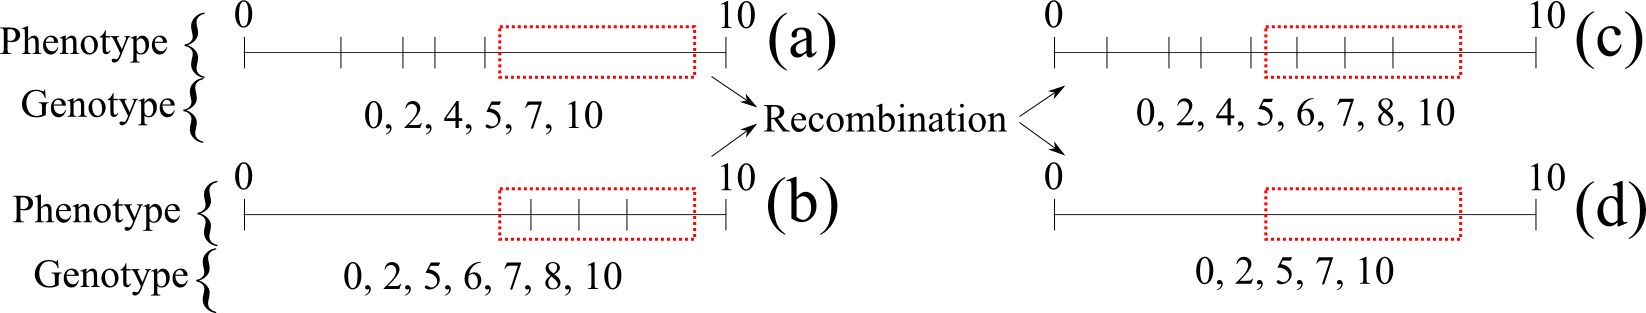
\includegraphics[width=2.5in]{emptyxover}
\caption{An example of a case where crossover can generate a solution with a small genotype. In this example, parents shown in (a) and (b) generate children in (c) and (d), one of which only contains a single segment. This violates a limitation of ADVANTG and prevents evaluation of the individual in (d) in subsequent development.}
\label{fig_sim}
\end{figure}

\subsection{Mutation Operator}
The mutation operator will randomly select one of two operations to perform: either add a gene or delete a gene. Addition of a gene will generate a gene randomly whithin the bounds of the phenotype and insert that gene into its proper position in the genotype. Deletion will select a gene at random and remove it from the genotype. Due to a limitation of the ADVANTG code, no individual with less than three segments in any dimension can be evalutated. Therefore, in the event that such an individual would be generated, no mutation is applied.

First, the mutation operator selects a random region. The region is chosen by choosing two points in the domain. The region is defined by all segments partially (or fully) enclosed by the two selected points. The mutation operator will randomly (with equal liklihood) choose to either sparcify or densify that region.

Sparcification and densification are each defined by a probability, $P_s$ and $P_d$ respectively. In practice, these probabilites are always set equal to one another to avoid issues of bloat.

\subsection{Termination}
Currently, the EA terminates after a user-specified wall time.

\section{Tentative Experimental Setup}
To illustrate the complexity of the problem, a simple use case was constructed. A 50 cm thick borated polyethylene (BPE) shield was modeled to shield a beam of parallel 2.45 MeV neutrons emitted toward a sodium iodide (NaI) detector. Another detector was placed 45 cm perpendicular to the beam from the edge of the shield to measure scattering effects. The FOM of both detectors is to be maximized simultaneously. To do this, a simple hill climber algorithm was implemented. The hill climber started by subdividing the spatial domain into a $5 \times 5 \times 5$ grid and running ADVANTG/MCNP. The segments in the $x$ direction were then increased by 5 and the simulation was re-run. The segments in the $x$ direction were increased by 5 again the simulation was re-run again. This was repeated until the $x$ subdivisions equaled to 100. The best (determined by the sum of the FOM of both detectors) was then selected as the optimal and then the same was repeated in the $y$ direction while holding the number of segments in $x$ and $z$ constant. Finally, the number of segments in the $z$ direction was optimized in a similar fashion. The fitness over this process is plotted in Fig.~\ref{fig:fitness_xyz}. The entire hill climber was run a second time in the same manner, except the ordering was reversed: $z$ was optimized first, followed by $y$ and then $x$ last. These results are plotted in Fig.~\ref{fig:fitness_zyx}. The optimal result in the $x \rightarrow y \rightarrow z$ direction was $30 \times 5 \times 50$ which resulted in a FOM of 1993.4 min$^{-1}$. The second run, produced an optimal result of $20 \times 5 \times 35$ which resulted in a FOM of 2112.1 min$^{-1}$.
\begin{figure}[!t]
  \centering
  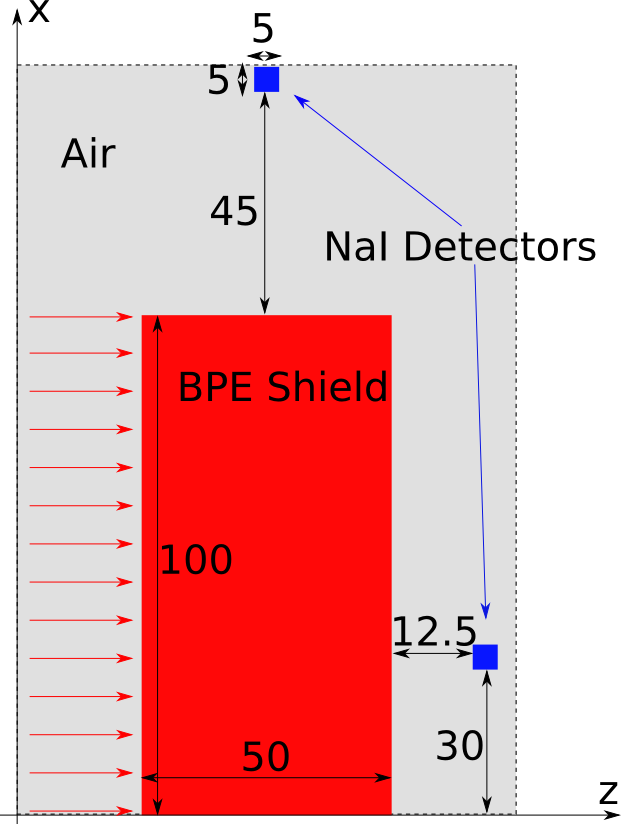
\includegraphics[width=2.5in]{probsetup}
  \caption{Problem setup (all units in cm).}
  \label{probsetup}
\end{figure}

\section{Tentative Results}
Charts!

\section{Tentative Discussion}
Wowzers!

\section{Current Challenges}
They're hard!

\section{Planned Work}
Working on it!


% An example of a floating figure using the graphicx package.
% Note that \label must occur AFTER (or within) \caption.
% For figures, \caption should occur after the \includegraphics.
% Note that IEEEtran v1.7 and later has special internal code that
% is designed to preserve the operation of \label within \caption
% even when the captionsoff option is in effect. However, because
% of issues like this, it may be the safest practice to put all your
% \label just after \caption rather than within \caption{}.
%
% Reminder: the "draftcls" or "draftclsnofoot", not "draft", class
% option should be used if it is desired that the figures are to be
% displayed while in draft mode.
%
%\begin{figure}[!t]
%\centering
%\includegraphics[width=2.5in]{myfigure}
% where an .eps filename suffix will be assumed under latex, 
% and a .pdf suffix will be assumed for pdflatex; or what has been declared
% via \DeclareGraphicsExtensions.
%\caption{Simulation results for the network.}
%\label{fig_sim}
%\end{figure}

% Note that the IEEE typically puts floats only at the top, even when this
% results in a large percentage of a column being occupied by floats.


% An example of a double column floating figure using two subfigures.
% (The subfig.sty package must be loaded for this to work.)
% The subfigure \label commands are set within each subfloat command,
% and the \label for the overall figure must come after \caption.
% \hfil is used as a separator to get equal spacing.
% Watch out that the combined width of all the subfigures on a 
% line do not exceed the text width or a line break will occur.
%
%\begin{figure*}[!t]
%\centering
%\subfloat[Case I]{\includegraphics[width=2.5in]{box}%
%\label{fig_first_case}}
%\hfil
%\subfloat[Case II]{\includegraphics[width=2.5in]{box}%
%\label{fig_second_case}}
%\caption{Simulation results for the network.}
%\label{fig_sim}
%\end{figure*}
%
% Note that often IEEE papers with subfigures do not employ subfigure
% captions (using the optional argument to \subfloat[]), but instead will
% reference/describe all of them (a), (b), etc., within the main caption.
% Be aware that for subfig.sty to generate the (a), (b), etc., subfigure
% labels, the optional argument to \subfloat must be present. If a
% subcaption is not desired, just leave its contents blank,
% e.g., \subfloat[].


% An example of a floating table. Note that, for IEEE style tables, the
% \caption command should come BEFORE the table and, given that table
% captions serve much like titles, are usually capitalized except for words
% such as a, an, and, as, at, but, by, for, in, nor, of, on, or, the, to
% and up, which are usually not capitalized unless they are the first or
% last word of the caption. Table text will default to \footnotesize as
% the IEEE normally uses this smaller font for tables.
% The \label must come after \caption as always.
%
%\begin{table}[!t]
%% increase table row spacing, adjust to taste
%\renewcommand{\arraystretch}{1.3}
% if using array.sty, it might be a good idea to tweak the value of
% \extrarowheight as needed to properly center the text within the cells
%\caption{An Example of a Table}
%\label{table_example}
%\centering
%% Some packages, such as MDW tools, offer better commands for making tables
%% than the plain LaTeX2e tabular which is used here.
%\begin{tabular}{|c||c|}
%\hline
%One & Two\\
%\hline
%Three & Four\\
%\hline
%\end{tabular}
%\end{table}


% Note that the IEEE does not put floats in the very first column
% - or typically anywhere on the first page for that matter. Also,
% in-text middle ("here") positioning is typically not used, but it
% is allowed and encouraged for Computer Society conferences (but
% not Computer Society journals). Most IEEE journals/conferences use
% top floats exclusively. 
% Note that, LaTeX2e, unlike IEEE journals/conferences, places
% footnotes above bottom floats. This can be corrected via the
% \fnbelowfloat command of the stfloats package.




%\section{Conclusion}
%The conclusion goes here.




% conference papers do not normally have an appendix


% use section* for acknowledgment
\section*{Acknowledgment}


The authors would like to thank...





% trigger a \newpage just before the given reference
% number - used to balance the columns on the last page
% adjust value as needed - may need to be readjusted if
% the document is modified later
%\IEEEtriggeratref{8}
% The "triggered" command can be changed if desired:
%\IEEEtriggercmd{\enlargethispage{-5in}}

% references section

% can use a bibliography generated by BibTeX as a .bbl file
% BibTeX documentation can be easily obtained at:
% http://mirror.ctan.org/biblio/bibtex/contrib/doc/
% The IEEEtran BibTeX style support page is at:
% http://www.michaelshell.org/tex/ieeetran/bibtex/
\bibliographystyle{IEEEtran}
% argument is your BibTeX string definitions and bibliography database(s)
\bibliography{IEEEabrv,./references}
%
% <OR> manually copy in the resultant .bbl file
% set second argument of \begin to the number of references
% (used to reserve space for the reference number labels box)
%\begin{thebibliography}{1}

%\bibitem{IEEEhowto:kopka}
%H.~Kopka and P.~W. Daly, \emph{A Guide to \LaTeX}, 3rd~ed.\hskip 1em plus
%  0.5em minus 0.4em\relax Harlow, England: Addison-Wesley, 1999.
%
%\end{thebibliography}




% that's all folks
\end{document}


